\section{Entornos de escritorio libres}
\subsection{¿Qué es un escritorio?}
\frame{
	\frametitle{¿Qué es un escritorio?}
	\begin{center}
		
\includegraphics[height=3cm,width=4cm]{./imgs/escritorio.jpg}
	\end{center}
  Conjunto de software que ofrece al usuario un entorno amigable con barras e
iconos con los que lanzar a ejecutar programas.

}

\subsection{GNOME}
\frame
{
	\begin{center}
		Un vistazo rápido a GNOME 2.12
		
\includegraphics[width=8.8cm]{./imgs/gnome-2_12.jpg}
	\end{center}	
}
\subsection{KDE}
\frame
{
	\begin{center}
		Un vistazo rápido a KDE 3.5.2
		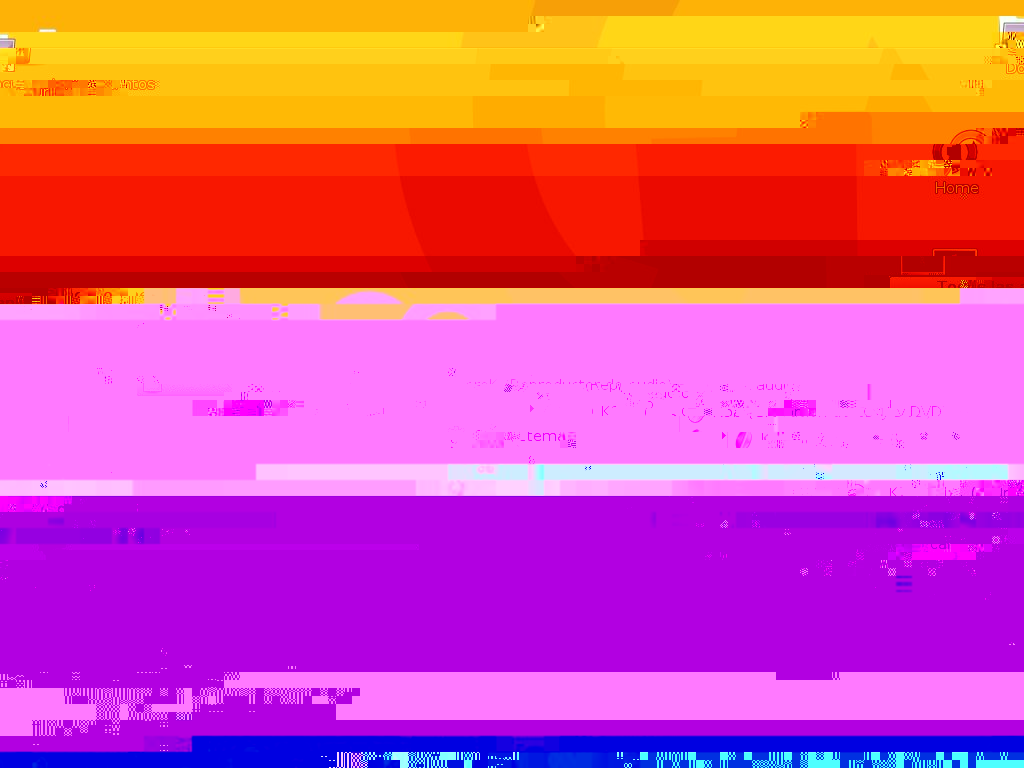
\includegraphics[width=8.8cm]{./imgs/pantallazoBardinux.jpg}
	\end{center}	
}
\subsection{Otros}
\frame
{
	\begin{center}
		\begin{tabular}{cc}
			\begin{tabular}c
		
\includegraphics[height=3cm,width=4cm]{./imgs/enlightenment.jpg} \\ Enlightenment
			\end{tabular} &
			\begin{tabular}c
		
\includegraphics[height=3cm,width=4cm]{./imgs/xfce.jpg} \\ XFCE
			\end{tabular} \\
			\begin{tabular}c
		
\includegraphics[height=3cm,width=4cm]{./imgs/afterstep.jpg} \\ AfterStep 
			\end{tabular} &
			\begin{tabular}c
		
\includegraphics[height=3cm,width=4cm]{./imgs/twm.jpg} \\ TWM 
			\end{tabular}
		\end{tabular}
	\end{center}	

}

